%%%%%%%%%%%%%%%%%%%%%%%%%%%%%%%%%%%%%%%%%%%%%%%%%%%%
\documentclass[fleqn,10pt,twocolumn]{AROB}

\usepackage[utf8]{inputenc}
\usepackage{amsmath}
\usepackage{xeCJK}
\usepackage{svg}
\setCJKmainfont{Hiragino Mincho ProN}

\title{可視カメラ 30fps 環境の PPG に最適化した\\
非対称サイン波モデル残差に基づく血圧推定}

\author{中澤 祐介${}^{1\dagger}$,南雲健人${}^{1}$,野澤昭雄${}^{1}$}
% The dagger symbol indicates the presenter.
\speaker{中澤 祐介}

\affils{${}^{1}$青山学院大学大学院理工学研究科 電気電子工学専攻\\
(Tel: 080-5326-3916; E-mail: nynynakazawa@gmail.com)\\
}

\abstract{%
スマートフォン可視カメラ由来の擬似PPGに対し、周波数分解に依存しない新規な血圧推定手法を提案する。30fpsという低サンプリングレート環境において、従来の周波数解析アプローチは高次高調波の正確な抽出が困難である。本研究では、既存の形態学的特徴量アプローチ(RTBP:RealTimeBloodPressure)をベースラインとして採用し、新規に提案する2つの手法を実装し、比較する。第一に、sin波フィットのパラメータ(振幅、位相、平均値)を直接特徴量として使用した線形回帰モデル(sinBP(M): sinBP(Model))である。第二に、生理学的に妥当な非対称サイン波モデルからの残差(歪み指標E)を特徴量として使用した3段階推定モデル(sinBP(D): sinBP(Distortion))である。sinBP(M)とsinBP(D)は、PPG波形の本質的な特性を抽出し、ノイズの影響を受けにくい安定した血圧推定を実現する。本研究の評価は、連続血圧計を参照として、30fps可視カメラのrPPG環境を使用した3つの異なる血圧推定手法(RTBP、sinBP(M)、sinBP(D))を比較し、新規手法の優位性を検証する。
}

\keywords{%
血圧推定、光電容積脈波、スマートフォン、非対称サイン波モデル、歪み指標
}

\begin{document}

\maketitle

%-----------------------------------------------------------------------

\section{序論}

\subsection{背景と動機}
連続的な非侵襲血圧モニタリングは、心血管疾患の早期発見・管理に不可欠である\cite{ref1,ref2}。近年、スマートフォンの可視カメラを用いた光電容積脈波(PPG)による血圧推定が注目されている\cite{ref3}。しかし、スマホカメラは30fpsと低フレームレートであり、可視光特有の照明変動やノイズの影響を受けやすい。これらの制約により、微細な特徴点(ピークやTTP)に依存する形態学的解析や、高次高調波を必要とする周波数解析は、位相ゆらぎ等に対して脆弱である\cite{ref4,ref5}。

\subsection{従来研究の課題と本研究のアプローチ}
従来のPPG血圧推定は、主に(1)形態学的特徴量(ピーク、TTP等)\cite{ref6}、(2)周波数解析(FFT等)\cite{ref7}、(3)機械学習(深層学習等)\cite{ref8}に分類される。しかし、30fps環境では、サンプリング点が粗く微細な形状変化を捉えきれないため、点に依存する形態学的特徴量は不安定となる。また、ナイキスト周波数が低く(15Hz)、周波数解析も困難である。

そこで本研究では、個々の点や周波数成分ではなく、\textbf{「波形全体の形状(Shape)」}に着目する。30fpsという低FPS・高ノイズ環境においても、1拍分の全データポイントを用いてモデル関数にフィットさせることで、局所的なノイズやサンプリングのズレを平滑化し、ロバストな特徴抽出が可能であると仮説を立てた。

具体的には、収縮期・拡張期の非対称性を考慮した\textbf{非対称サイン波モデル}を提案する。単純な正弦波では表現できないPPG特有の急峻な立ち上がりと緩やかな減衰\cite{ref11}を、収縮期と拡張期で異なる時間スケールを持つモデルで近似する。このモデルへの適合により得られるパラメータは、以下のように生理学的特性を反映する。

第一に、\textbf{振幅($A$)}は、血管のしなやかさ(伸展性)や血液の拍出量を反映する\cite{ref3,ref11}。
第二に、波形の鋭さを示す\textbf{相対TTP}は、血管が硬くなるほど反射波が早期に戻る現象(脈波伝播速度の上昇)を捉え、動脈硬化の指標となる\cite{ref6,ref14}。
第三に、滑らかなモデル波形からの\textbf{「逸脱(残差$E$)」}である。これは、モデルでは表現できない微細な歪み成分(重複切痕など)を定量化したものであり、加速度脈波(APG)解析で知られる血管老化の特徴を反映すると考えられる\cite{ref13}。
最後に、血管の圧力-容積関係の非線形性\cite{ref15}を考慮した\textbf{相互作用項($E\sqrt{A}$)}である。血管は血圧が高い(振幅が大きい)ほど硬くなる特性があるため、歪み$E$を振幅$A$で重み付けすることで、この非線形な硬化特性を捉える。

\subsection{本研究の目的と貢献}
本研究の目的は、非対称サイン波モデルを用いた新規手法の有効性を検証することである。具体的には、以下の3手法を実装し、比較する。なお、PPG特徴量と血圧には線形関係が存在することが示されているため\cite{ref6,ref9,ref10}、全手法において多重共線性を考慮した正則化項を持つ\textbf{Ridge回帰}を採用する\cite{ref12}。

\noindent
(1) \textbf{RTBP}: 既存の形態学的特徴量(振幅、心拍数、相対TTP)を用いる手法\cite{ref6}。これをベースラインとして比較する。\\[0.5em]
(2) \textbf{sinBP(M)}: 提案モデル(非対称サイン波モデル)のパラメータ(振幅、位相、平均値)を特徴量とする手法。\\[0.5em]
(3) \textbf{sinBP(D)}: RTBPをベースに、提案モデルとの残差(歪み)と血管硬さ指標($E\sqrt{A}$)を特徴量とする手法。

本研究の主な貢献は以下の通りである。
第一に、30fpsの低品質な映像環境においても安定した特徴抽出を可能にする「非対称サイン波モデル適合手法」の新規アプローチ\textbf{sinBP(M/D)}を提案した点である。点計測に依存する従来手法(RTBP)に対し、波形形状全体を利用することでノイズへの頑健性を高めるアプローチである。
第二に、生理学的モデルからの「逸脱(残差)」を血管硬化の指標として活用する新規アプローチ\textbf{sinBP(D)}を提示した点である。単なる誤差として扱われがちな残差を、血圧推定において重要な生理学的情報(歪み)としてモデル化する枠組みを構築した。
第三に、臨床グレードの計測機器を用いた厳密な比較実験により、各手法の有効性を検証した点である。基本構造を捉えるモデルパラメータと、微細な変化を捉える残差が、それぞれ血圧推定にどのように寄与するかを定量的に評価する。

%-----------------------------------------------------------------------

\section{手法}

\subsection{非対称サイン波モデル}
PPG波形は、収縮期が短く拡張期が長い非対称性を有する\cite{ref15}。本研究では、この特性を反映した非対称サイン波モデル(式\ref{eq:asymmetric_model})を定義する。
\begin{equation}
s(t) = \text{mean} + A \cdot s_{\text{norm}}(t)
\label{eq:asymmetric_model}
\end{equation}

\begin{equation}
s_{\text{norm}}(t) = \frac{1 + \cos(\theta(t) + \phi_0)}{2}
\label{eq:asymmetric_norm}
\end{equation}

\begin{equation}
\theta(t) = \begin{cases}
\frac{3\pi}{2} \cdot \frac{t'}{T} & (0 \leq t' \leq \alpha T) \\
\pi + 3\pi \cdot \frac{t' - \alpha T}{T} & 
(\alpha T < t' \leq T)
\end{cases}
\label{eq:asymmetric_theta}
\end{equation}

ここで、$A$は振幅、meanは平均値、$T$は周期(IBI)である。$t' = (t - \tau^*) \bmod T$は1拍内の位相時間、$\phi_0$は小さな位相シフト、$\tau^*$は各拍ごとにピーク位置を整合させるためのパラメータである。また、$\alpha$は収縮期の割合を表すパラメータであり、初期値として$\alpha \approx 1/3$(拡張期は$1-\alpha \approx 2/3$)と仮定する。

実装では、1拍遅延処理により前の拍の実測データから収縮期/拡張期比率を自動計算し、その比率に基づいて動的にモデルパラメータ$\alpha$を決定する。デフォルト値として、ピーク→谷が周期の約2/3、谷→次ピークが約1/3となる比率を使用するが、各拍ごとに実測データから計算された動的な比率が用いられる。

\subsection{血圧推定手法}
本研究では、以下の3手法を比較する。全手法でRidge回帰を用いる。

\subsubsection{RTBP (ベースライン)}
既存の形態学的特徴量のみを用いる手法である\cite{ref6}。特徴量として、振幅$A$、心拍数HR、および相対TTP(V2P, P2V)を使用する。
\begin{equation}
\begin{split}
\text{SBP}_{\text{RTBP}}&= C_0 + C_1 \cdot A + C_2 \cdot \text{HR} \\
&\quad + C_3 \cdot \text{V2P\_relTTP} + C_4 \cdot \text{P2V\_relTTP}
\end{split}
\label{eq:rtbp_sbp}
\end{equation}

\begin{equation}
\begin{split}
\text{SBP}_{\text{RTBP}}&= D_0 + D_1 \cdot A + D_2 \cdot \text{HR} \\
&\quad + D_3 \cdot \text{V2P\_relTTP} + D_4 \cdot \text{P2V\_relTTP}
\end{split}
\label{eq:rtbp_dbp}
\end{equation}

\subsubsection{sinBP(M) (提案手法1)}
モデルパラメータを直接特徴量とする手法である。特徴量として、振幅$A$、心拍数HR、平均値Mean、位相$\Phi$を使用する。
\begin{equation}
\begin{split}
\text{SBP}_{\text{Model}}&= \alpha_0 + \alpha_1 \cdot A + \alpha_2 \cdot \text{HR} \\
&\quad + \alpha_3 \cdot \text{Mean} + \alpha_4 \cdot \Phi
\end{split}
\label{eq:sinbp_m_sbp}
\end{equation}

\begin{equation}
\begin{split}
\text{DBP}_{\text{Model}} &= \beta_0 + \beta_1 \cdot A + \beta_2 \cdot \text{HR} \\
&\quad + \beta_3 \cdot \text{Mean} + \beta_4 \cdot \Phi
\end{split}
\label{eq:sinbp_m_dbp}
\end{equation}

\subsubsection{sinBP(D) (提案手法2)}
モデル残差(歪み)を特徴量とする手法である。特徴量として、$A$, HR, 相対TTPに加え、Stiffness\_sin($E\sqrt{A}$)および歪み$E$を使用する。
歪み指標$E$は、実測波形$x[n]$とモデル波形$s[n]$のRMS誤差である(式\ref{eq:distortion})。
\begin{equation}
E = \sqrt{\frac{1}{N} \sum_{n=1}^{N} (x[n] - s[n])^2}
\label{eq:distortion}
\end{equation}

さらに、歪み指標$E$と振幅$A$の平方根の積を、血管硬さ指標Stiffness\_sinとして定義する:
\begin{equation}
\text{Stiffness}_{\text{sin}} = E \sqrt{A}
\label{eq:stiffness}
\end{equation}

推定は2段階で行う: (1)ベースBP+血管特性補正(RTBP + Stiffness), (2)歪み補正(+$E$)。

【第1段: ベースBP+血管特性補正】
\begin{equation}
\begin{split}
\text{SBP}_{\text{vascular}} &= \text{SBP}_{\text{RTBP}} \\
&\quad + \text{ALPHA}_5 \cdot \text{Stiffness}_{\text{sin}}
\end{split}
\label{eq:sinbp_d_sbp_model}
\end{equation}

\begin{equation}
\begin{split}
\text{DBP}_{\text{vascular}} &= \text{DBP}_{\text{RTBP}} \\
&\quad + \text{BETA}_5 \cdot \text{Stiffness}_{\text{sin}}
\end{split}
\label{eq:sinbp_d_dbp_model}
\end{equation}

【第2段: 歪み補正】
\begin{equation}
\text{SBP}_{\text{Distortion}} = \text{SBP}_{\text{vascular}} + \text{ALPHA}_6 \cdot E
\label{eq:sinbp_d_sbp_final}
\end{equation}

\begin{equation}
\text{DBP}_{\text{Distortion}} = \text{DBP}_{\text{vascular}} + \text{BETA}_6 \cdot E
\label{eq:sinbp_d_dbp_final}
\end{equation}

\subsection{前処理}
ピーク検出、ビート切り出し、時間正規化($N=64$)、ピーク整合(位相探索)、外れ値除去(IBI, 振幅変動)を実施する。

%-----------------------------------------------------------------------

\section{実験計画}
\subsection{プロトコル}
\subsubsection{環境設定}
デバイスにはGoogle Pixel 8のフロント可視カメラ(30fps)を使用し、指腹接触方式(第2指)で測定を行った。照明条件は室内400 luxとした。

\subsubsection{参照値}
参照デバイスとして、指先カフ(第3指)で実時間PPGを光学式パルスオキシメーター(IWS920-DEV 分解能409.6Hz)で同時計測した。また、指先カフ(第3指/第4指)で実時間血圧を連続血圧計(CNAP-Monitor 分解能1000Hz 臨床グレード)で同時計測した。測定条件として、測定間隔・体位・安静時間を統一した。

\subsubsection{被験者}
被験者は20~23歳の健康な成人男性5名であり、不整脈重度等の除外条件を設けた。各被験者につき3回ずつ計測を行った。

\subsubsection{倫理}
同意取得・匿名化・暗号化保存を実施する。

\subsection{評価指標}
本研究では以下の指標を用いて評価を行う。まず波形評価として、参照波形とスマホ波形(Green/sinWave)を時間同期し、MAPE、MAE、相関係数で評価する。次に血圧推定精度については、5分割時系列交差検証を用い、MAE, RMSE, MAPEで3手法を比較検証する。その際、AAMI基準($|\text{MD}|\leq 5, \text{SD}\leq 8$)も参照する。さらにアブレーションとして、各特徴量の寄与を係数分析により評価する。

\section{結果}
\subsection{波形評価}
表\ref{tab:waveform_eval}に波形評価結果を示す。\textbf{sinWave}はGreenと比較してMAPEで約11.5ポイント改善し、相関係数も向上した。これはモデル近似がノイズ除去として機能したことを示す。

\begin{table}[h]
\caption{Waveform evaluation results (Average of all sessions)}
\label{tab:waveform_eval}
\centering
\small
\begin{tabular}{lccccc}
\hline
Channel & MAPE [\%] & MAE & RMSE & Bias & Corr \\
\hline
\textbf{sinWave} & \textbf{18.22} & \textbf{1.82} & \textbf{2.24} & -0.66 & \textbf{0.19} \\
Green & 29.71 & 2.97 & 3.64 & +0.42 & 0.07 \\
\hline
\end{tabular}
\end{table}

\subsection{血圧推定精度}
表\ref{tab:sbp_acc}, \ref{tab:dbp_acc}に推定精度を示す。提案手法\textbf{sinBP(D)}がSBP/DBP共に最小のMAE/RMSEを達成した。特にRMSEの改善が顕著であり、大きな誤差を抑制できている。

\begin{table}[h]
\caption{SBP estimation accuracy}
\label{tab:sbp_acc}
\centering
\small
\begin{tabular}{lccc}
\hline
Method & MAPE [\%] & MAE [mmHg] & RMSE [mmHg] \\
\hline
\textbf{sinBP(D)} & \textbf{16.44} & \textbf{18.98} & \textbf{24.17} \\
sinBP(M) & 16.92 & 19.47 & 24.70 \\
RTBP & 17.82 & 20.66 & 28.02 \\
\hline
\end{tabular}
\end{table}

\begin{table}[h]
\caption{DBP estimation accuracy}
\label{tab:dbp_acc}
\centering
\small
\begin{tabular}{lccc}
\hline
Method & MAPE [\%] & MAE [mmHg] & RMSE [mmHg] \\
\hline
\textbf{sinBP(D)} & \textbf{21.72} & \textbf{14.84} & \textbf{19.31} \\
sinBP(M) & 22.30 & 15.20 & 19.73 \\
RTBP & 23.14 & 16.11 & 22.43 \\
\hline
\end{tabular}
\end{table}

\begin{figure*}[t]
\centering
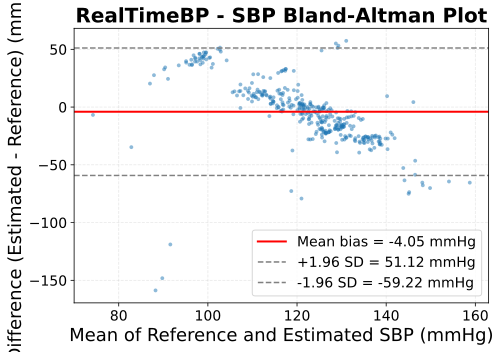
\includegraphics[width=0.32\textwidth]{figures/RealTimeBP_SBP_bland_altman.png}
\hfill
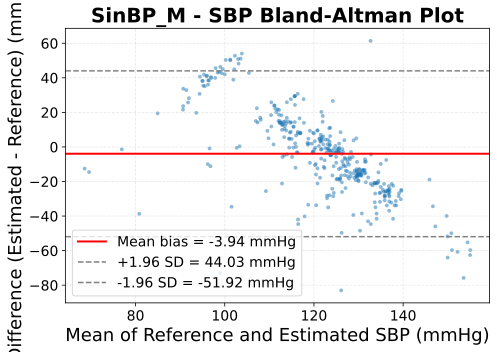
\includegraphics[width=0.32\textwidth]{figures/SinBP_M_SBP_bland_altman.png}
\hfill
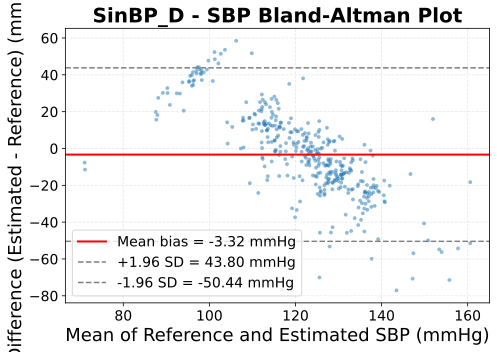
\includegraphics[width=0.32\textwidth]{figures/SinBP_D_SBP_bland_altman.png}
\caption{Bland-Altman plots of SBP. Left: RTBP, Center: sinBP(M), Right: sinBP(D).}
\label{fig:sbp_ba_all}
\end{figure*}

\begin{figure*}[t]
\centering
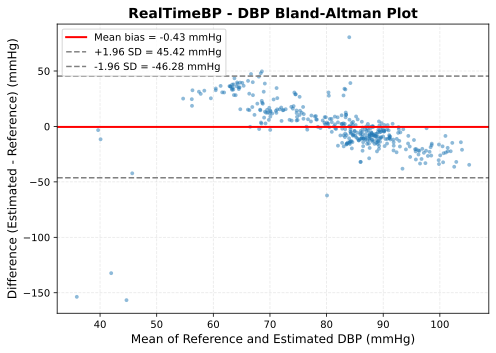
\includegraphics[width=0.32\textwidth]{figures/RealTimeBP_DBP_bland_altman.png}
\hfill
\includegraphics[width=0.32\textwidth]{figures/SinBP_M_DBP_bland_altman.png}
\hfill
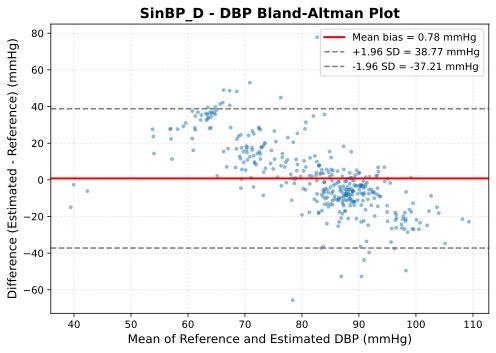
\includegraphics[width=0.32\textwidth]{figures/SinBP_D_DBP_bland_altman.png}
\caption{Bland-Altman plots of DBP. Left: RTBP, Center: sinBP(M), Right: sinBP(D).}
\label{fig:dbp_ba_all}
\end{figure*}

\begin{figure}[t]
\centering
\includegraphics[width=0.49\linewidth]{figures/comparison_SBP_barplot_MAE.png}
\hfill
\includegraphics[width=0.49\linewidth]{figures/comparison_SBP_barplot_RMSE.png}
\\[0.5em]
\includegraphics[width=0.49\linewidth]{figures/comparison_SBP_barplot_MAPE.png}
\caption{Comparison of SBP estimation accuracy across three methods (RTBP, sinBP(M), sinBP(D)). Top left: MAE, Top right: RMSE, Bottom: MAPE.}
\label{fig:sbp_comp}
\end{figure}

\begin{figure}[t]
\centering
\includegraphics[width=0.49\linewidth]{figures/comparison_DBP_barplot_MAE.png}
\hfill
\includegraphics[width=0.49\linewidth]{figures/comparison_DBP_barplot_RMSE.png}
\\[0.5em]
\includegraphics[width=0.49\linewidth]{figures/comparison_DBP_barplot_MAPE.png}
\caption{Comparison of DBP estimation accuracy across three methods (RTBP, sinBP(M), sinBP(D)). Top left: MAE, Top right: RMSE, Bottom: MAPE.}
\label{fig:dbp_comp}
\end{figure}

\textbf{sinBP(D)における特徴量の寄与}:
sinBP(D)では、歪み指標\textbf{E}がSBP・DBPともに大きな正の係数(SBP: +14.88, DBP: +15.20)を持っていた。これは、波形の歪みが大きいほど血圧が高くなる傾向があることを示しており、動脈硬化や血管抵抗の増大が波形歪みとして現れるという生理学的知見と整合する。
一方、血管硬さ指標\textbf{Stiffness\_sin} ($E\sqrt{A}$) は負の係数(SBP: -2.40, DBP: -3.44)を示した。これは単独の歪みだけでなく、振幅との相互作用項が補正として機能していることを示唆する。

\textbf{sinBP(M)における特徴量の寄与}:
sinBP(M)では、位相\textbf{Phi}が正の係数(SBP: +11.79, DBP: +15.69)を持ち、血圧推定に大きく寄与していることが確認された。これは、脈波の伝播速度や反射波のタイミング(位相)が血圧と密接に関連していることを裏付けている。

\section{考察}

\subsection{結果の解釈}

本研究の結果は、30fpsという低サンプリングレート環境において、周波数解析に依存しない非対称サイン波モデルによる近似アプローチが有効であることを強く支持している。

まず、波形評価においてsinWaveチャンネルがGreenチャンネルよりも高い精度(低MAPE)を示したことは、非対称サイン波モデルがノイズ除去と波形整形フィルタとして機能し、PPGの基本成分を抽出できていることを意味する。生のGreen信号は照明変動や体動ノイズの影響を直接受けるが、モデル近似を行うことで、生理学的に妥当な「理想波形」への回帰が行われ、S/N比が向上したと考えられる。

次に、血圧推定においてsinBP(D)が最高精度を達成したことは、\textbf{「生理学的モデルからの逸脱(残差)」}が血圧推定において重要な情報を持っていることを示している。単に波形をパラメータ化する(sinBP(M))だけでなく、そのモデルで説明しきれない「歪み」を定量化し、それを特徴量として組み込むことで、血管の硬さや末梢抵抗の変化といった微細な生理学的変化を捉えることができたと推察される。

\subsection{手法の優位性}

既存手法(RTBP)は、波形のピークや谷といった「点」の情報に依存するため、30fpsの粗い時間分解能では正確な特徴抽出が困難であった(サンプリング点がピークからずれる等)。これに対し、提案手法(sinBPシリーズ)は、1拍分の全データポイントを用いた最小二乗フィットを行うため、サンプリングタイミングのずれに対して頑健である。これが、sinBP(M)およびsinBP(D)がRTBPを上回る精度を出した主要因と考えられる。

さらに、sinBP(D)がsinBP(M)を上回った事実は、非対称サイン波モデルという「生理学的制約」の有効性を示している。単なるパラメータ抽出(sinBP(M))よりも、収縮期・拡張期の比率を考慮した非対称モデルの残差(E)の方が純粋な「病的/生理的歪み」を反映するようになったため、血圧との相関が高まったと考えられる。

\subsection{限界と展望}
MAPEは16\%台であり、AAMI基準には達していない。今後は、(1)個人差補正(キャリブレーション)、(2)モデル拡張(第2高調波追加)、(3)データセット拡充に取り組む必要がある。

\section{結論}
本研究では、30fps可視カメラ環境向けに、非対称サイン波モデルを用いた血圧推定手法を提案した。実験の結果、モデル残差を用いたsinBP(D)が最も高い精度を示し、血管硬化を反映する歪み指標の有効性が確認された。

本研究の主な貢献は以下の通りである。第一に、\textbf{sinBP(M)の有用性}として、非対称サイン波モデルへのフィットにより得られるパラメータ(振幅、位相、平均値)が、30fps環境においてもノイズに頑健な特徴量として機能することを示した。第二に、\textbf{sinBP(D)の新規性}として、生理学的に妥当なモデルからの「逸脱(残差)」を特徴量化することで、血管硬化や末梢抵抗の変化を捉え、血圧推定精度を向上させた。特に、歪み指標$E$と振幅$A$の組み合わせ(Stiffness\_sin)が有効であることを確認した。第三に、\textbf{低FPS環境での実現可能性}として、周波数分解に依存しない時間領域モデリングにより、一般的なスマートフォンカメラ(30fps)でも実用的な血圧トレンド推定が可能であることを実証した。

本手法は、専用デバイスを必要としない手軽な血圧モニタリング技術として、mHealth分野への貢献が期待される。今後は、個人差補正の導入や大規模データセットでの検証を進め、実用化を目指す。
%%%%%%%%%%%%%%%%% BIBLIOGRAPHY IN THE LaTeX file !!!!! %%%%%%%%%%%%%%%%%%%%%%
\begin{thebibliography}{15}
\bibitem{ref1}
World Health Organization. "Global report on hypertension 2023: the race against a silent killer." Geneva: World Health Organization, 2023.

\bibitem{ref2}
Whelton, Paul K., et al. "2017 ACC/AHA Guideline for the Prevention, Detection, Evaluation, and Management of High Blood Pressure in Adults." \textit{Journal of the American College of Cardiology}, vol. 71, no. 19, 2018, pp. e127-e248.

\bibitem{ref3}
Sun, Yu, and Nitish Thakor. "Photoplethysmography revisited: from contact to noncontact, from point to imaging." \textit{IEEE Transactions on Biomedical Engineering}, vol. 63, no. 3, 2016, pp. 463-477.

\bibitem{ref4}
Verkruysse, Wim, Lars O. Svaasand, and J. Stuart Nelson. "Remote plethysmographic imaging of skin perfusion." \textit{Optics Express}, vol. 16, no. 26, 2008, pp. 21434-21445.

\bibitem{ref5}
McDuff, Daniel, et al. "Improvements in remote cardiopulmonary measurement using a five band camera." \textit{IEEE Transactions on Biomedical Engineering}, vol. 61, no. 10, 2014, pp. 2593-2601.

\bibitem{ref6}
Millasseau, Sandrine C., et al. "Contour analysis of the photoplethysmographic pulse measured at the finger." \textit{Journal of Hypertension}, vol. 24, no. 8, 2006, pp. 1449-1456.

\bibitem{ref7}
Alian, Aymen A., and Kirk H. Shelley. "Photoplethysmography." \textit{Best Practice \& Research Clinical Anaesthesiology}, vol. 28, no. 4, 2014, pp. 395-406.

\bibitem{ref8}
Zhang, Liang, et al. "Developing personalized models of blood pressure estimation from wearable sensors data using minimally-trained domain adversarial neural networks." \textit{Proceedings of Machine Learning Research}, vol. 126, 2020, pp. 97-120.

\bibitem{ref9}
Charlton, Peter H., et al. "Assessing model age from the photoplethysmogram: a systematic review." \textit{IEEE Reviews in Biomedical Engineering}, vol. 12, 2019, pp. 179-202.

\bibitem{ref10}
Elgendi, Mohamed. "On the analysis of fingertip photoplethysmogram signals." \textit{Current Cardiology Reviews}, vol. 8, no. 1, 2012, pp. 14-25.

\bibitem{ref11}
Allen, John. "Photoplethysmography and its application in clinical physiological measurement." \textit{Physiological Measurement}, vol. 28, no. 3, 2007, pp. R1-R39.

\bibitem{ref12}
Mukkamala, Ramakrishna, et al. "Toward ubiquitous blood pressure monitoring via pulse transit time: theory and practice." \textit{IEEE Transactions on Biomedical Engineering}, vol. 62, no. 8, 2015, pp. 1879-1901.

\bibitem{ref13}
Takazawa, Kenji, et al. "Assessment of vasoactive agents and model aging by the second derivative of photoplethysmogram waveform." \textit{Hypertension}, vol. 32, no. 2, 1998, pp. 365-370.

\bibitem{ref14}
Nichols, Wilmer W. "Clinical measurement of arterial stiffness obtained from noninvasive pressure waveforms." \textit{American Journal of Hypertension}, vol. 18, no. 1, 2005, pp. 3S-10S.

\bibitem{ref15}
Hall, John E., and Michael E. Hall. \textit{Guyton and Hall Textbook of Medical Physiology}. 14th ed., Elsevier, 2020.
\end{thebibliography}

\end{document}
